The \texttt{OpenNN} training strategy is composed by three algorithms: 
an initialization, a main and a refinement training algorithms. 
In this section we study the software model of the \lstinline"TrainingStrategy" class.

\subsubsection{Classes}

In order to construct a software model for the training strategy, a few
things need to be taken into account. 

As we have seen, a training strategy is composed of three different training algorithms. 
On the other hand, some training algoritms use one-dimensional optimization for finding the optimal training rate. 
Therefore, the most important classes in the training strategy are:

\begin{description}
\item[Training algorithm] The class \lstinline"TrainingAlgorithm" represents a single training algorithm.

\item[Training rate algorithm] The class \lstinline"TrainingRateAlgorithm" represents the one-dimensional optimization algorithm for the training rate.

\item[Training strategy] The class \lstinline"TrainingStrategy" represents a complete training strategy, 
and it is composed of initialization, main and refinement training algorithms. 
\end{description}

\subsubsection{Associations}

The associations among the concepts described above are the following:

\begin{description}
\item[Training algorithm - Training rate algorithm] A training algorithm might require a training rate algorithm during the optimization process.

\item[Training strategy - Training algorithm] A training strategy might be composed of different training algorithms.
\end{description}

Figure \ref{AssociationDiagramTrainingStrategy} shows the UML class diagram for
the training strategy with some of the derived classes included.

\begin{figure}[h!]
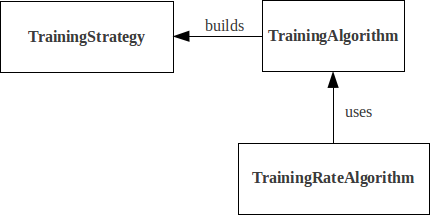
\includegraphics[width=0.7\textwidth]{training_strategy/training_stategy_association_diagram.png}
\caption{Association diagram for the training strategy.}\label{AssociationDiagramTrainingStrategy}
\end{figure}


\subsubsection{Derived classes}\index{derived class, object oriented programming}

The next task is then to establish which classes are abstract and
to derive the necessary concrete classes to be added. Let us then examine the classes we have so far:

\begin{description}

\item[Training algorithm] The class \lstinline"TrainingAlgorithm" is abstract, because it does not
represent a training algorithm for a performance function of a neural network.

The concrete training algorithm classes included with \texttt{OpenNN} are \lstinline"RandomSearch", \lstinline"GradientDescent", \lstinline"NewtonMethod", \lstinline"ConjugateGradient", \lstinline"QuasiNewtonMethod" and \lstinline"EvolutionaryAlgorithm".

\item[Training rate algorithm] This class is concrete, because it has several one-dimensional methods implemented. 

\item[Training strategy] The class \lstinline"TrainingStrategy" is concrete, since it is composed by concrete initialization, main and refinement training algorithms. 

\end{description}

Figure \ref{TrainingStrategyDerivedClassDiagram} shows the UML class diagram for the training strategy with some of the derived classes included.

\begin{figure}[h!]
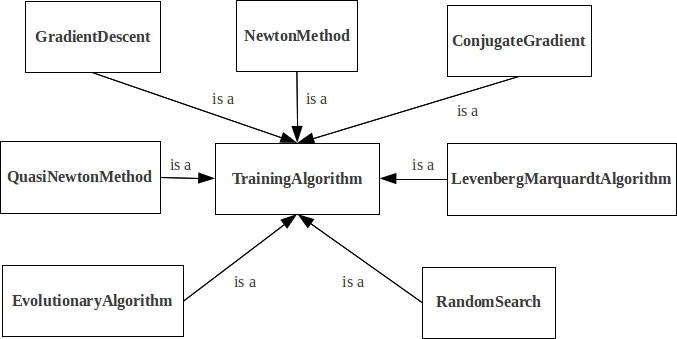
\includegraphics[width=1.1\textwidth]{training_strategy/training_strategy_derived_class_diagram.png}
\caption{Derived classes related to the training strategy.}\label{TrainingStrategyDerivedClassDiagram}
\end{figure}

\subsubsection{Attributes and operations}\index{attribute, object oriented programming}
\index{operation, object oriented programming}

\begin{description}

\item[Training algorithm] A training algorithm has the following attributes:

\begin{itemize}
\item[-] A relationship to a performance functional. In C++ this is implemented as a pointer to a performance functional object.
\item[-] A set of training operators.
\item[-] A set of training parameters.
\item[-] A set of stopping criteria.
\end{itemize}

It performs the following operations:

\begin{itemize}
\item[-] Train a neural network.
\end{itemize}

\item[Training rate algorithm] A training rate algorithm has the following attributes:

\begin{itemize}
\item[-] A relationship to a performance functional. 
\item[-] The training rate algorithm method to use.
\item[-] A set of parameters.
\end{itemize}

It performs the following operations:

\begin{itemize}
\item[-] Calculate the training rate.
\end{itemize}

\item[Training strategy] A training strategy has the following attributes:

\begin{itemize}
\item[-] A relationship to a performance functional. 
\item[-] A pointer to an initialization training algorithm.
\item[-] A pointer to a main training algorithm.
\item[-] A pointer to a refinement training algorithm.
\item[-] A flag for using the initialization training algorithm.
\item[-] A flag for using the main training algorithm.
\item[-] A flag for using the refinement training algorithm.
\end{itemize}

It performs the following operations:

\begin{itemize}
\item[-] Calculate the training rate.
\end{itemize}

\end{description}
